% ==============================================================
% SECCIÓN 5: TRABAJO FUTURO — CONTROL REPETITIVO
% ==============================================================

% --- Slide 18: Análisis a baja velocidad ---
\begin{frame}{Extensión: Análisis de Límites a Baja Velocidad}
    \textbf{Problema identificado:} el observador de BEMF falla cuando $\omega \rightarrow 0$,
    ya que $\mathbf{e} = K_e\,\omega\,\mathbf{s}(\theta) \rightarrow \mathbf{0}$ y la señal se
    hunde en el ruido del ADC ($\sigma \approx 50\,\text{mA}$, 12-bit).

    \vspace{0.2cm}

    \begin{columns}[T]
    \begin{column}{0.52\textwidth}
        \textbf{Se caracterizó en simulación:}
        \begin{itemize}
            \item Resolución del encoder vs.\ velocidad: por debajo de $\sim\!15$ rpm el encoder
                  queda ``congelado'' entre muestras $\rightarrow$ el observador debe interpolar.
            \item Ripple baseline del M2PC a \{5, 10, 20, 60\} rpm con encoder ideal
                  (velocidad impuesta, sin PI).
        \end{itemize}
        \vspace{0.2cm}
        \textbf{Conclusión:} el rizo crece sustancialmente a baja velocidad $\rightarrow$
        motiva extender el controlador para este régimen.
    \end{column}
    \begin{column}{0.45\textwidth}
        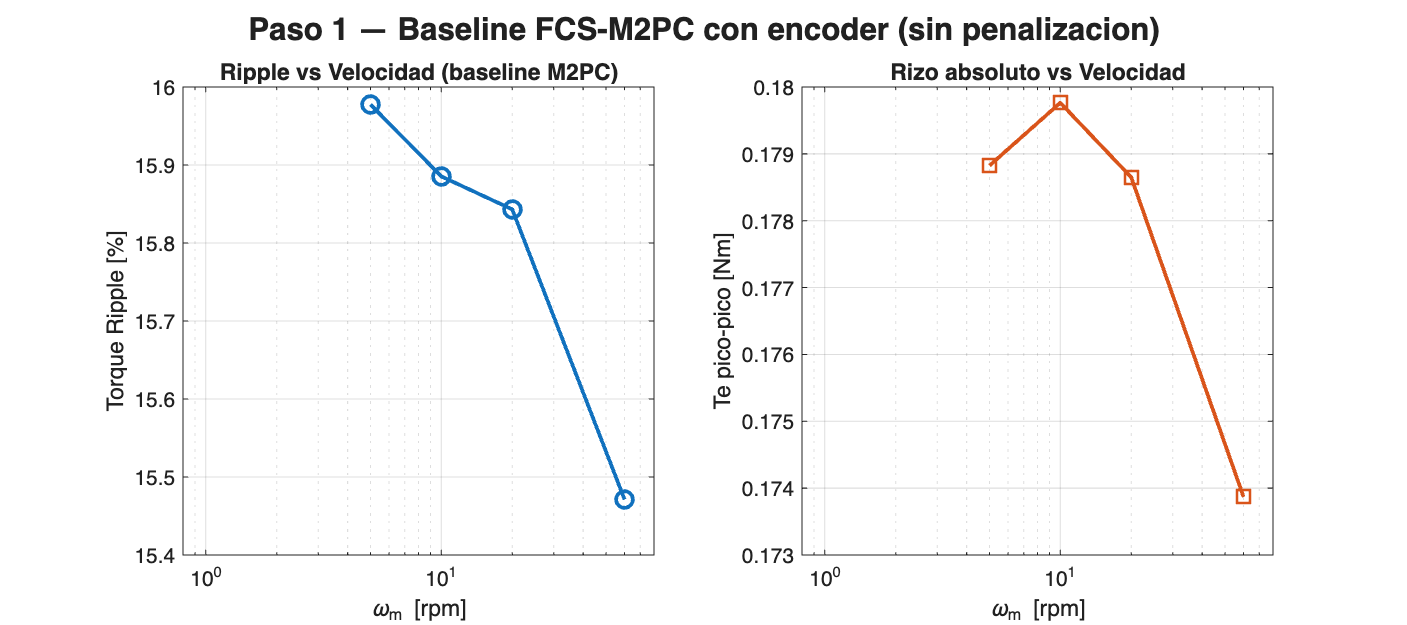
\includegraphics[width=\linewidth]{fig/baseline_ripple_vs_speed.png}
        {\tiny Ripple de par vs.\ velocidad — M2PC con encoder 2048\,PPR}
    \end{column}
    \end{columns}
\end{frame}

% --- Slide 19: Limitaciones actuales ---
\begin{frame}{¿Qué Falta? Fuentes de Rizo que ADALINE No Elimina}
    El ADALINE corrige el \textit{model mismatch} de BEMF, pero quedan fuentes de rizo \textbf{que no son error de BEMF}:
    
    \vspace{0.3cm}
    
    \begin{columns}[T]
    \begin{column}{0.48\textwidth}
        \begin{alertblock}{Fuentes residuales}
            \begin{itemize}
                \item \textbf{Cogging torque:} función de $\theta$, independiente de corriente. Armónicos 6to, 12vo.
                \item \textbf{Dead-time del inversor:} distorsiona el voltaje aplicado. Armónicos 5to/7mo.
                \item \textbf{Discretización M2PC:} $\rho$ finito $\rightarrow$ error de cuantización.
            \end{itemize}
        \end{alertblock}
    \end{column}
    \begin{column}{0.48\textwidth}
        \begin{exampleblock}{Propiedad común}
            Todas son \textbf{perturbaciones periódicas} con frecuencias múltiplos de la frecuencia eléctrica.
            
            \vspace{0.3cm}
            
            $\rightarrow$ Candidatas perfectas para \textbf{Control Repetitivo (RC)}.
        \end{exampleblock}
    \end{column}
    \end{columns}
\end{frame}

% --- Slide 19: Control Repetitivo ---
\begin{frame}{Control Repetitivo: Rechazo de Disturbios Periódicos}
    \textbf{Principio del Modelo Interno:} para rechazar una perturbación periódica de período $T$, el controlador debe contener el generador de señal periódica:
    \begin{equation}
        C_{RC}(z) = \frac{Q(z)\,z^{-N}}{1 - Q(z)\,z^{-N}} \cdot z^p \cdot G_f(z), \qquad N = T/T_s
    \end{equation}
    
    Esto provee \textbf{ganancia infinita en todos los armónicos} simultáneamente.
    
    \vspace{0.3cm}
    
    \begin{columns}[T]
    \begin{column}{0.48\textwidth}
        \textbf{Arquitectura propuesta:}
        \begin{enumerate}
            \item \textbf{ADALINE} (feedforward): corrige errores de BEMF $\rightarrow$ elimina rizo grueso.
            \item \textbf{RC} (feedback): compensa rizo residual periódico $\rightarrow$ elimina cogging, dead-time.
        \end{enumerate}
    \end{column}
    \begin{column}{0.48\textwidth}
        \textbf{Conexión ADALINE $\rightarrow$ RC:}
        \begin{itemize}
            \item Los pesos del ADALINE revelan el \textbf{espectro del motor}.
            \item Esto informa el diseño de $Q(z)$ y $G_f(z)$ del RC.
            \item Esquema RC selectivo: atacar solo los armónicos que ADALINE no puede eliminar.
        \end{itemize}
    \end{column}
    \end{columns}
\end{frame}

% --- Slide 20: Roadmap ---
\begin{frame}{Roadmap de la Investigación}
    \begin{center}
    \begin{tikzpicture}[
        node distance=0.4cm and 0.3cm,
        phase/.style={draw, rounded corners, minimum width=2.8cm, minimum height=1cm, align=center, font=\small},
        done/.style={phase, fill=ForestGreen!20, draw=ForestGreen},
        curr/.style={phase, fill=YellowOrange!25, draw=YellowOrange},
        future/.style={phase, fill=gray!15, draw=gray},
        arrow/.style={-{Stealth[length=2mm]}, thick}
    ]
        \node[done] (f0) {\textbf{Fase 0}\\ADALINE Offline\\$\checkmark$ Completada};
        \node[done, right=of f0] (f1) {\textbf{Fase 1}\\ADALINE Online\\$\checkmark$ Completada};
        \node[curr, right=of f1] (f2) {\textbf{Fase 2}\\Encoder + baja\\velocidad};
        \node[future, right=of f2] (fq) {\textbf{???}\\Por definir};

        \draw[arrow] (f0) -- (f1);
        \draw[arrow] (f1) -- (f2);
        \draw[arrow] (f2) -- (fq);

        % Anotaciones debajo
        \node[below=0.3cm of f0, font=\tiny, align=center, text=ForestGreen] {40 params\\RMSE 0.0009};
        \node[below=0.3cm of f1, font=\tiny, align=center, text=ForestGreen] {LMS online\\$\sim$9\% $\downarrow$ ripple};
        \node[below=0.3cm of f2, font=\tiny, align=center, text=YellowOrange] {2048 PPR\\Análisis $\omega$ bajo};
        \node[below=0.3cm of fq, font=\tiny, align=center, text=gray] {Next steps\\(reunión hoy)};
    \end{tikzpicture}
    \end{center}
    
    \vspace{0.5cm}
    
    \textbf{Contribución principal:} Arquitectura en tres capas (ADALINE offline $\rightarrow$ ADALINE online $\rightarrow$ RC) que ataca el rizo de par desde la causa (BEMF) hasta el efecto residual (perturbaciones periódicas), con complejidad computacional compatible con DSP en tiempo real.
\end{frame}

% --- Slide 21: Conclusiones ---
\begin{frame}{Conclusiones Parciales}
    \begin{enumerate}
        \item El \textbf{ADALINE con base de Fourier} iguala la precisión de una NN profunda ($\sim$25k params) con solo \textbf{40 parámetros}, entrenado en \textbf{12 ms} vs.\ 30 s.
        
        \vspace{0.2cm}
        
        \item El \textbf{ADALINE online (LMS)} converge en $<$2 revoluciones eléctricas y alcanza el mismo rendimiento que el entrenamiento offline, demostrando capacidad de \textbf{auto-calibración}.
        
        \vspace{0.2cm}
        
        \item La integración ADALINE + FCS-M2PC reduce el rizo de par en $\sim$\textbf{9\%} respecto al modelo trapezoidal convencional, sin requerir datos previos del motor.
        
        \vspace{0.2cm}
        
        \item Los coeficientes de Fourier del ADALINE proveen una \textbf{representación interpretable} del motor que sirve como puente natural hacia el \textbf{Control Repetitivo}.
    \end{enumerate}
    
    \vspace{0.3cm}
    
    \begin{center}
        \textbf{Siguiente paso:} Integrar RC plug-in para atacar cogging torque y dead-time --- las fuentes de rizo que el ADALINE no puede eliminar por diseño.
    \end{center}
\end{frame}